% Research draft v0.1 for discussion (not for citation / submission).
% Compile: pdflatex main && bibtex main && pdflatex main && pdflatex main
\documentclass[11pt]{article}

\usepackage[margin=1.05in]{geometry}
\usepackage[T1]{fontenc}
\usepackage{lmodern}
\usepackage{microtype}
\usepackage{amsmath,amssymb}
\usepackage{booktabs}
\usepackage{graphicx}
\usepackage{tikz}
\usetikzlibrary{arrows.meta,positioning,fit,calc}
\usepackage{xcolor}
\usepackage{hyperref}
\usepackage{enumitem}
\usepackage{caption}
\usepackage{natbib}

\hypersetup{
  colorlinks=true,
  linkcolor=blue!50!black,
  citecolor=blue!50!black,
  urlcolor=blue!50!black
}

\definecolor{warnbg}{HTML}{F8E6E0}
\definecolor{okbg}{HTML}{E7F2EA}

\newcommand{\task}[1]{\texttt{#1}}
\newcommand{\Pone}{\textsc{P1}}
\newcommand{\Ptwo}{\textsc{P2}}
\newcommand{\Pthree}{\textsc{P3}}

\title{When the World Changes but the Score Does Not:\\
A Counterfactual Audit of Computer-Use Agents}
\author{Vinh Duc Tran\\
Hanoi University of Science and Technology\\
\texttt{vinh.td@hust.edu.vn} \textit{(placeholder)}}
\date{Research draft v0.1 --- 27 August 2026}

\begin{document}
\maketitle

\begin{abstract}
Computer-use agents are typically evaluated by whether they complete a
task under a fixed rubric. Task completion does not establish that the
score \emph{identifies} which environment state produced the success.
We audit this property with paired counterfactual episodes: a controlled
intervention changes a pre-registered determining set $D$ while the
instruction, interface, rubric, and harness stay fixed. We separately
code \emph{tracking} (does the final answer follow $D$?) and
\emph{score invariance} (does the judge move when the gold moves?).

Under a frozen Stage-4 protocol on MyPCBench, three computer-use systems
(Claude Opus~4.6, GPT-5.5, Qwen3.5-35B-A3B) all track a loyalty-tier
intervention on \task{retrieval-f001} while the judge stays at $100$.
Claude and GPT also track an aggregation intervention
(\(\approx\$4872\to\$400\)) with unchanged scores.
A Qwen3.5-9B size ablation tracks both tasks; an exploratory
Qwen3.8-Flash run does too. Score invariance does \emph{not} hold on
every completed Qwen pair. Incomplete trajectories are coded as
technical failures, not as ``does not track.''
On Claude \task{preference-inference-f018}, the judge stays at $100$
while tracking of the joint $D$ is only partial---the one current cell
in which success conceals incomplete tracking.

The claim is not that agents ignore personal data, nor that invariant
scores are always wrong. It is that a scalar task score is an
insufficient identifier of counterfactual world-state. For CUA
development this is operational, not only diagnostic: a stable
leaderboard number is not evidence that the agent is latched onto a
particular personal record, and a high score can conceal two
incompatible worlds---or an incomplete read of a joint determining set.
Paired gold-moving checks belong beside completion scores; conventional
CUA leaderboards do not perform them.
\end{abstract}

\section{Introduction}

Computer-use agents (CUAs) act on screenshots, click and type, and are
scored on whether they finish the task~\citep{jang2026mypcbench,xie2024osworld}.
That evaluation answers a capability question: \emph{did the trajectory
satisfy the rubric?} It does not answer a reliability question:

\begin{quote}
\textit{When a task-relevant state in the world is counterfactually
changed, does the agent's reported outcome change with it---and would
the score have told us?}
\end{quote}

These are different questions. Consider a loyalty dashboard. An
intervention changes Gold Voyager / $38{,}450$ miles into Silver Voyager
/ $8{,}620$. If the agent then reports Silver / $8{,}620$, it tracked
the state. If the judge remains $100$, the score did not identify which
world produced the success. Conversely, if the agent still reports Gold
while scoring $100$, the score conceals a tracking failure.

We therefore treat CUA evaluation as a \emph{counterfactual audit}, not
as another benchmark sweep. For each frozen task we run a baseline
environment $E^0$ and an intervened environment $E^1=I(E^0)$, with $I$
locked before confirmatory runs. The same instruction, rubric, and agent
interface are applied to both. From each completed pair we read two
quantities that the locked protocol already distinguished:

\begin{itemize}[leftmargin=1.3em,itemsep=0.25em]
  \item \textbf{Tracking} (behavioral DV): does the final answer follow
        the determining set $D$ of the intervention?
  \item \textbf{Score invariance} (evaluator diagnostic): is
        $|S^1-S^0|$ small relative to the gold change, given that both
        episodes completed and a guest probe shows that gold moved?
\end{itemize}

The object of study is interactive computer-use agents under controlled
SQL interventions.

\paragraph{Contributions.}
\begin{enumerate}[leftmargin=1.3em,itemsep=0.3em]
  \item A counterfactual audit that separates tracking from task scoring,
        with explicit coding of technical failure vs.\ behavioral
        evidence.
  \item A frozen intervention protocol (eligibility, seed, SQL, DVs)
        on MyPCBench~\citep{jang2026mypcbench}, using real $1280\times 800$
        screenshots and guest-side probes that gold moved.
  \item Cross-agent evidence on two clean tasks, a within-family 9B
        ablation, an exploratory Flash check, and one Claude cell in
        which score invariance coexists with incomplete tracking.
\end{enumerate}

\paragraph{What we do not claim.}
We do not claim that agents fail to use personal data. On the clean
pairs they often \emph{do} track. We do not claim model-generality from
two or three systems. We do not
promote held-out or confounded task IDs after seeing outcomes.
The Phase-A memo locked these restrictions before the GPT and Qwen cells.

\section{Related work}

\paragraph{Computer-use evaluation.}
Desktop and web agents are scored in interactive
environments~\citep{xie2024osworld,zhou2024webarena,koh2024visualwebarena}.
MyPCBench~\citep{jang2026mypcbench} additionally seeds a coherent
persona across 17 logged-in apps and 184 tasks, and reports rubric
scores under a computer+bash tool surface. Those leaderboards measure
completion. They do not intervene on the persona state that the rubric
treats as gold and then ask whether the score still identifies the
world.

\paragraph{Reliability beyond accuracy.}
A score can be high for reasons other than the intended mechanism.
If the object of interest is state-sensitive behavior, a scalar that is
invariant to a gold-moving intervention is not a sufficient statistic
for that object.

\paragraph{Counterfactuals as identification.}
The design is a paired intervention~\citep{pearl2009causality}: same
task, same agent, one pre-registered state change. Unrelated-task
comparisons cannot separate agent behavior from task difficulty.

\section{Counterfactual audit}

\subsection{Two DVs, not one}

For frozen task $t$, let $E_t^0$ be the seeded guest and
$E_t^1 = I_t(E_t^0)$ the guest after a locked SQL patch on determining
set $D_t$. The same agent $A$, instruction $T$, screenshot size, and
judge $J$ yield trajectories $\tau^0=A(T,E_t^0)$ and $\tau^1=A(T,E_t^1)$.
A guest probe after $I_t$ must show that gold moved; otherwise the pair
is not an intervention.

From each completed $\tau$ we extract
$G$ (the task-relevant quantities in the \emph{final answer}) and
$S=J(\tau)$ (rubric score in $\{0,\ldots,100\}$).

\paragraph{\Ptwo{} --- tracking (primary behavioral DV).}
Code $\mathrm{track}=1$ iff $G^1$ matches $D_t$ on $E_t^1$ and $G^0$
matches $D_t$ on $E_t^0$, using the pre-registered answer fields (tier
and miles; combined refund; asserted GME shares and YES bet; etc.).
Do not code tracking from $S$.

\paragraph{\Pone{} --- score invariance (evaluator diagnostic).}
If both episodes reach \texttt{DONE}, the probe shows gold moved, and
$|S^1-S^0|$ is small relative to the gold change, the judge did not
detect the intervention. This is \emph{not} a claim that the agent is
reliable. It is a claim about $J$.

\paragraph{Why invariance can be expected.}
Eligibility required channel-invariant rubrics that do not pin a
dollar/tier gold in the instruction. Under that screen, a judge that
scores ``did the agent use the apps and report \emph{a} loyalty tier?''
can award $100$ to both Gold and Silver. Score invariance is then a
property we \emph{built into} the sample, not a surprise about
Claude's internals. It remains scientifically useful: it shows that
published-style success is compatible with two incompatible worlds.

\paragraph{Two patterns that matter.}
\begin{description}[leftmargin=1.6em,style=nextline,itemsep=0.35em]
  \item[Type A.] Track and score-invariant.
        The agent read the new world; the score cannot tell Gold from
        Silver. This is an evaluation gap.
  \item[Type B.] Incomplete tracking and score-invariant.
        The agent did not follow the full $D$; the score still looks
        like success. This is a reliability gap the leaderboard hides.
\end{description}
Type~A is currently the replicated pattern. Type~B is currently one
Claude cell (\task{f018}). They must not be averaged into one ``agents
are unreliable'' slogan.

\subsection{Coding incomplete episodes}

A GUI abort, step-limit without \texttt{DONE}, missing tool XML, or
screenshot-decode crash is \Pthree{}: \texttt{technical\_failure} /
\texttt{failure}. It is not $\mathrm{track}=0$ and not a refutation of
\Pone{}. Empty trajectories and host crashes are infrastructure, not
DVs.

\subsection{Frozen protocol}

Selection was pre-registered on eligibility A--E (channel-invariant;
mapped SQLite; \texttt{cua\_required} false; no LibreOffice/GUI
artifact; instruction does not pin a dollar gold) and a seed
\texttt{20260826} sample, $k\le 3$ per evidence type:
\[
184 \;\to\; 10\text{ eligible} \;\to\; 8\text{ confirmatory sample}.
\]
Four sample members are confounded on this seed and stay in the sample
un-run for attribution:
\task{retrieval-f029}, \task{retrieval-f030},
\task{aggregation-f018}, \task{preference\_inference-f004}.
Two identifiable reserves (\task{retrieval-f003}, \task{retrieval-f016})
were not promoted after seeing outcomes.

Runnable Stage-4 IDs: \task{retrieval-f001}, \task{aggregation-f003},
\task{preference\_inference-f018}, \task{counterfactual-f004}.
SQL patches are locked in \texttt{cf/stage4\_locked.json}. We do not
invent a different patch after seeing an answer.

\section{Experimental setup}

\paragraph{Environment.}
Official MyPCBench QEMU guest, persona
\texttt{michael.scott@dundermifflin.com} (canonical identity),
screenshots $1280\times 800$.
Interventions are SQL on guest SQLite; the agent is not told that a
patch occurred. Judge: Anthropic \texttt{per\_step} when available
(auxiliary).

\paragraph{Agents.}
\begin{itemize}[leftmargin=1.3em,itemsep=0.2em]
  \item Claude: \texttt{claude\_cuabash} / \texttt{claude-opus-4-6}
        (confirmatory Stage~4).
  \item GPT: \texttt{openai\_cuabash} / \texttt{gpt-5.5}
        (exploratory transfer; same SQL).
  \item Qwen paper CUA: \texttt{qwen\_cuabash} /
        \texttt{qwen/qwen3.5-35b-a3b} via a hosted OpenAI-compatible
        endpoint (OpenRouter). Local HPC 27B+vLLM was abandoned after
        infrastructure failure and is \emph{not} a result.
  \item Qwen3.5-9B: size ablation under the same XML CUA interface,
        \task{f001}+\task{f003} only.
  \item Qwen3.8-Flash: exploratory cross-version check, same two tasks.
        It does not replace 35B-A3B as the paper Qwen id.
\end{itemize}

\section{Results}

\begin{figure}[t]
\centering
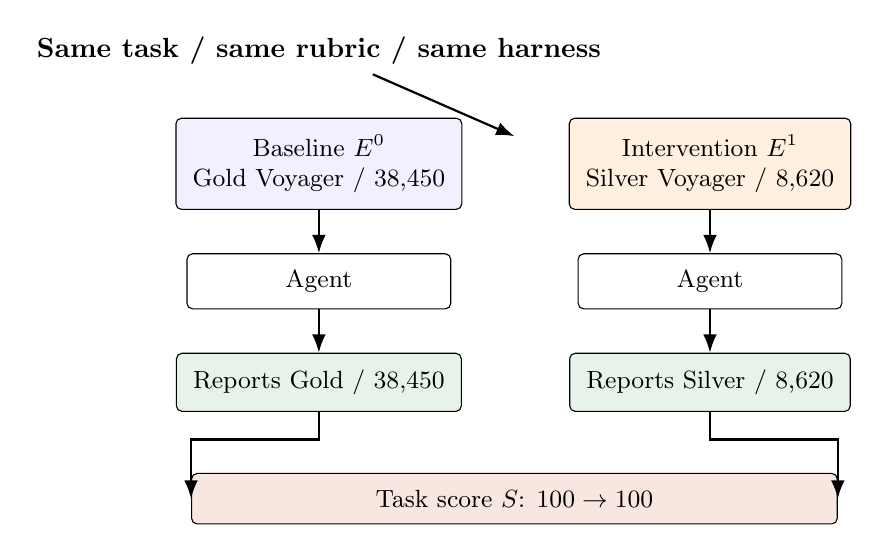
\begin{tikzpicture}[
  font=\small,
  box/.style={draw, rounded corners=2pt, align=center, inner sep=6pt, minimum width=3.35cm},
  arr/.style={-{Latex}, thick}
]
\node[font=\bfseries] (top) {Same task / same rubric / same harness};
\node[box, below=0.55cm of top, fill=blue!6] (b0) {Baseline $E^0$\\Gold Voyager / $38{,}450$};
\node[box, right=1.35cm of b0, fill=orange!12] (b1) {Intervention $E^1$\\Silver Voyager / $8{,}620$};
\node[box, below=0.55cm of b0] (a0) {Agent};
\node[box, below=0.55cm of b1] (a1) {Agent};
\node[box, below=0.55cm of a0, fill=okbg] (g0) {Reports Gold / $38{,}450$};
\node[box, below=0.55cm of a1, fill=okbg] (g1) {Reports Silver / $8{,}620$};
\node[box, fill=warnbg, below=1.15cm of $(g0)!0.5!(g1)$, minimum width=8.2cm] (s)
  {Task score $S$: $100 \rightarrow 100$};
\draw[arr] (top) -- ($(b0)!0.5!(b1)+(0,0.35)$);
\draw[arr] (b0) -- (a0);
\draw[arr] (b1) -- (a1);
\draw[arr] (a0) -- (g0);
\draw[arr] (a1) -- (g1);
\draw[arr] (g0.south) -- ++(0,-0.35) -| (s.west);
\draw[arr] (g1.south) -- ++(0,-0.35) -| (s.east);
\end{tikzpicture}
\caption{\textbf{Type~A audit (schematic of \task{retrieval-f001}).}
The world state changes by an order of magnitude; the agent tracks it;
the conventional score need not move. Caption, not architecture
diagram: world changed; behavior tracked; score was not an identifier.}
\label{fig:audit}
\end{figure}

\subsection{How to read the tables}

Table~\ref{tab:scores} is the scan table: only \texttt{DONE}+\texttt{DONE}
pairs, with $\Delta S=S^1-S^0$ in its own column. Primary Type~A rows
have $\Delta S=0$. The two Qwen size/exploratory \task{f003} rows are
the completed pairs where the judge \emph{does} move.
Table~\ref{tab:fail} keeps incomplete cells in view; they are not in
any invariance denominator. Writer scripts that mark a crashed cell as
\texttt{ok} are overridden by the trajectory (Qwen 35B \task{f018} CF
is \texttt{PREDICT\_CRASH}).

\begin{table}[t]
\centering
\small
\setlength{\tabcolsep}{4.2pt}
\begin{tabular}{@{}ll rr r c l@{}}
\toprule
Agent & Task & $S^0$ & $S^1$ & $\Delta S$ & Track & Pattern \\
\midrule
\multicolumn{7}{@{}l}{\textit{Primary Type~A --- invariance $5/5$, $\Delta S=0$}} \\
Claude & \task{f001} & 100 & 100 & $0$ & yes & Type A \\
Claude & \task{f003} & 80 & 80 & $0$ & yes & Type A \\
GPT-5.5 & \task{f001} & 100 & 100 & $0$ & yes & Type A \\
GPT-5.5 & \task{f003} & 50 & 50 & $0$ & yes & Type A \\
Qwen 35B-A3B & \task{f001} & 100 & 100 & $0$ & yes & Type A \\
\midrule
\multicolumn{7}{@{}l}{\textit{Type~B (one cell; not in the $5/5$ rate)}} \\
Claude & \task{f018} & 100 & 100 & $0$ & partial & Type B \\
\midrule
\multicolumn{7}{@{}l}{\textit{Size ablation / exploratory --- not pooled into $5/5$}} \\
Qwen 9B & \task{f001} & 80 & 80 & $0$ & yes & Type A \\
Qwen 9B & \task{f003} & 50 & 80 & $+30$ & yes & tracks; not invariant \\
Qwen Flash & \task{f001} & 100 & 100 & $0$ & yes & Type A \\
Qwen Flash & \task{f003} & 80 & 100 & $+20$ & yes & tracks; not invariant \\
\bottomrule
\end{tabular}
\caption{Valid \texttt{DONE}+\texttt{DONE} pairs. Gold moved on every
row (\task{f001}: Gold/$38450\to$Silver/$8620$; \task{f003}:
$\approx\$4872\to\$400$; \task{f018}: GME $85\to 0$ and OM YES
$200$ active$\to$settled). $S$ is the auxiliary rubric score.
Primary invariance is $5/5$ with $\Delta S=0$ (35B \task{f003} has no
valid CF). 9B and Flash \task{f003} show that $\Delta S=0$ is not
automatic once tracking succeeds.}
\label{tab:scores}
\end{table}

\begin{table}[t]
\centering
\small
\setlength{\tabcolsep}{4pt}
\begin{tabular}{@{}ll l l@{}}
\toprule
Agent & Task & Why excluded from $\Delta S$ & Last status \\
\midrule
Claude & \task{f004} & no baseline \texttt{DONE} & $S$: $0\to 87$; out of inference \\
GPT-5.5 & \task{f018} & no \texttt{DONE} either cell & not ``does not track'' \\
GPT-5.5 & \task{f004} & 1099 still cited after patch & $87\to 87$; not attributed \\
Qwen 35B-A3B & \task{f003} & CF not \texttt{DONE} (3 attempts) & missing, not negative \\
Qwen 35B-A3B & \task{f018} & CF screenshot decode crash & technical failure \\
Qwen 35B-A3B & \task{f004} & step limit, both sides & failure \\
\bottomrule
\end{tabular}
\caption{Cells that do not enter tracking or invariance denominators.
Execution failure is not coded as $\mathrm{track}=0$.}
\label{tab:fail}
\end{table}

\subsection{Cross-agent Type~A on \task{f001}}
\label{sec:f001}

\task{retrieval-f001} is the cleanest cell. $I$ updates
\texttt{loyalty.\{status, miles, miles\_ytd\}} from Gold Voyager /
$38{,}450$ to Silver Voyager / $8{,}620$. Claude, GPT, and
Qwen3.5-35B-A3B each complete both episodes, report the new tier and
miles, and keep $S=100$. Figure~\ref{fig:audit} is this cell.

This is the strongest cross-agent result we have: three independent CUA
stacks, one locked SQL, Type~A. It is still one task and one evidence
type (\texttt{point\_field}).

\paragraph{Primary $k/n$.}
Across the frozen primary agents, there are five valid
\texttt{DONE}+\texttt{DONE} pairs on \task{f001}+\task{f003}
(35B-A3B~\task{f003} excluded). All five track $D$ and all five are
score-invariant: $5/5$ (Clopper--Pearson 95\% CI $[0.48,1.00]$).
We do not interpret the interval as a significance test. 9B
\task{f003} ($50\to 80$) and Flash \task{f003} ($80\to 100$) are
tracking-valid and \emph{score-sensitive}; they are not in this
denominator.

\subsection{Aggregation: \task{f003}}
\label{sec:f003}

$I$ rewrites filed 2023/2024 refunds so the combined gold moves
$4871.70 \to 400.00$ ($n_{\mathrm{filed}}=2$ held fixed; 2025
in-progress untouched). Claude tracks with $80\to 80$. GPT tracks with
$50\to 50$ (the absolute score is lower---the GPT answer missed
year-count rubric items---but \Pone{} still holds). Qwen3.5-35B-A3B
completes the baseline ($\approx\$4872$) and does not complete the CF
(attempt~1: 80-step scroll loop; later retry: FAIL / missing executable
tool call). That is missing evidence, not ``Qwen does not track \$400.''

Qwen3.5-9B tracks both sides. $S$ moves $50\to 80$, so this pair
supports tracking and \emph{rejects} a blanket invariance claim.
Qwen3.8-Flash likewise tracks; $S$ moves $80\to 100$. We report those
deltas rather than folding them into ``the same qualitative pattern.''

\subsection{Type~B: Claude \task{f018}}
\label{sec:f018}

The locked $D$ is a \emph{conjunction across two apps}: BatBucks GME
shares $85\to 0$ \emph{and} OddsMarket YES
$200/\texttt{active}\to 0/\texttt{settled}$. The instruction asks for a
GameStop-conviction rebalance (cost basis only). Claude's CF answer
tracks the stock conjunct (shares $=0$) and still asserts an active
YES $200$ bet. $S$ stays $100\to 100$. GPT and Qwen 35B did not produce
a valid CF \texttt{DONE}; we do not assign Type~B to them.

This is not ``the agent ignored personal data.'' It read BatBucks. The
gap is that $J$ can treat a coherent GME-conviction narrative as task
success without requiring both conjuncts of $D$ to be represented in
the final answer. Two structural features make that possible. First,
$D$ is multi-source: zeroing one database does not automatically
surface the other in the same screenshot. Second, the rubric is
advice-shaped rather than a pinned field check, so reporting ``lean
into GameStop'' can still pass after the YES position is gone. Type~A
tasks (\task{f001}, \task{f003}) ask for a quantity that lives in one
place; Type~B here is what a joint $D$ looks like when $J$ scores the
story, not each conjunct.

We therefore treat \task{f018} as a mechanism sketch, not a replicated
rate: a high score can conceal \emph{which subset} of $D$ produced the
answer. Replicating Type~B needs another completed pair on a joint
determining set---not another model on \task{f001}.

\subsection{What we refuse to convert into DVs}

Qwen 35B \task{f004}: both cells hit the step limit. Claude
\task{f004}: no baseline \texttt{DONE}. GPT \task{f018}: no actions /
no \texttt{DONE}. Qwen 35B \task{f018} CF: screenshot decode crash.
A hosted 35B interface layer can break XML tool emission; that is
harness/model-interface, not a tracking estimate.

\section{Discussion}

\subsection{The finding, stated narrowly}

On completed gold-moving pairs, agents \emph{can} track $D$ while $S$
stays put (Type~A), and---in one Claude cell---$S$ can stay put while
tracking of joint $D$ is incomplete (Type~B). A leaderboard number does
not tell a reader which of these occurred, nor which world the agent
saw. The $5/5$ primary count is a census of valid primary pairs, not
an estimate of Type~A over 184 tasks. 9B/Flash \task{f003} already
show that tracking does not imply $\Delta S=0$.

\subsection{Score invariance is not automatically a bug}

If $I$ changed a variable the rubric ignores, $S^0\approx S^1$ is
correct scoring. Our eligibility rule selected tasks whose instructions
do not pin the personal quantity, so Type~A is partly a statement about
$J$ under that screen. The operational implication is still sharp:
\emph{do not ship, rank, or select a CUA on a stable high score as if
that score identified a particular personal record.} A paired
gold-moving probe---same instruction, locked $I$, guest check that gold
moved, tracking coded from the answer---is the test that the
leaderboard omits. Type~B adds a second operational warning: even when
the agent used \emph{some} personal evidence, $J$ may not tell you
whether it used the whole determining set.

\subsection{Cross-agent and scale}

Three families on \task{f001} reduce the chance that Type~A is a Claude
artifact. 9B tracking both tasks reduces the chance that only the 35B-A3B
checkpoint can see the dashboard. Neither fact licenses a 184-task
sweep or a claim that size does not matter in general.

\subsection{What would actually scale the claim}

Paired-episode coding is already done: five primary pairs, all Type~A;
execution failures kept out of the denominator. A sixth CUA family
would not change that. If we scale, the target is more
\emph{independent} gold-moving tasks of the same design---to test
whether Type~A is systematic or an artifact of
\task{f001}/\task{f003}---plus item-level judge coding (whether $J$
ever mentions the manipulated numeral). That still cannot manufacture
Type~B replication we do not have.

\section{Limitations}

\begin{itemize}[leftmargin=1.3em,itemsep=0.35em]
  \item \textbf{N / generalizability.} This is an exhibited phenomenon
        on a frozen sample, not a population rate. Cross-agent Type~A
        is strongest on one task (\task{f001}). Reviewers should treat
        $5/5$ as a complete count of valid primary pairs, not as
        evidence that Type~A holds for CUA tasks in general.
  \item \textbf{Type~B} is one Claude cell on a joint $D$. GPT/Qwen CF
        episodes on the same task did not complete, so the mechanism
        (conjunction + advice-shaped rubric) is not yet cross-agent.
  \item \textbf{Score movement} on 9B/Flash \task{f003} already shows
        that \Pone{} is not universal even inside the Qwen family.
  \item \textbf{Hosted Qwen 35B} is not the abandoned local vLLM 27B
        stack. Tool-call failures may mix model and endpoint.
  \item \textbf{We evaluate agent systems} (\texttt{claude\_cuabash},
        \texttt{openai\_cuabash}, \texttt{qwen\_cuabash}), not isolated
        base models.
\end{itemize}

\section{Conclusion}

We audited computer-use agents by changing the world and holding the
task fixed. Conventional scores can remain compatible with two
incompatible persona states; agents may track the change, track it
only in part, or fail to finish the episode. Those three outcomes are
not interchangeable, and a scalar rubric score does not name which one
occurred. Counterfactual evaluation is a small complementary test:
intervene on $D$, require a guest probe that gold moved, code tracking
from the answer, and refuse to treat crashes as psychology. A completion
score is not a substitute for that check.

\bibliographystyle{plainnat}
\bibliography{refs}

\end{document}
